\begin{enumerate}[label=\thesection.\arabic*.,ref=\thesection.\theenumi]
\numberwithin{equation}{enumi}
\item The open loop transfer function of a unity feedback system is given by
\begin{align}
\label{eq:ee18btech11007_system}
 G(s)=\frac{\pi e^{-0.25s}}{s}
\end{align}
\item Find $\text{Re} \cbrak{G(\j \omega)}$ and $\text{Im} \cbrak{G(\j \omega)}$.
\\
\solution From \eqref{eq:ee18btech11007_system},
%
\begin{align}
G(j\omega)&=\frac{\pi}{\omega}(-\sin{0.25\omega}-j\cos{0.25\omega})
\\
\implies  \text{Re} \cbrak{G(\j \omega)}&=\frac{\pi}{\omega}(-\sin{0.25\omega}) 
\\
 \text{Im} \cbrak{G(\j \omega)}&=\frac{\pi}{\omega}(-j\cos{0.25\omega}) 
\end{align}
%
\item Sketch the Nyquist plot.
\\
\solution The Nyquist plot is a graph of $\text{Re} \cbrak{G(\j \omega)}$  vs $\text{Im} \cbrak{G(\j \omega)}$.
The following python code generates the Nyquist plot in Fig.  \ref{fig:ee18btech11007}
%
\begin{figure}[!h]
  \includegraphics[width=\columnwidth]{./figs/ee18btech11007.eps}
  \caption{}
  \label{fig:ee18btech11007}
\end{figure}
%
\item Find the point at which the Nyquist plot of G(s) passes through the negative real axis
\\
\solution  Nyquist plot cuts the negative real axis at $\omega $ for which 
\begin{align}
\angle G(\j\omega)=-\pi
\label{eq:ee18btech11007_system_neg_real}
\end{align}
From \eqref{eq:ee18btech11007_system},
\begin{align}
 G(\j\omega)&=\frac{\pi e^{-\frac{\j\omega}{4}}}{\j\omega} = \frac{\pi e^{-\j\brak{\frac{\omega}{4}+\frac{\pi}{2}}}}{\omega}
\\
\implies \angle{ G(\j\omega)} &= -\brak{\frac{\omega}{4}+\frac{\pi}{2}}
\label{eq:ee18btech11007_system_ang}
\end{align}
From \eqref{eq:ee18btech11007_system_ang} and \eqref{eq:ee18btech11007_system_neg_real}, 
\begin{align}
\frac{\omega}{4}+\frac{\pi}{2} &= \pi
\\
\implies \omega = 2\pi
\end{align}
Also, from \eqref{eq:ee18btech11007_system},
\begin{align}
\label{eq:ee18btech11007_system_mod}
\abs{ G(\j\omega)}&=\frac{\pi }{\abs{\omega}}
\\
\implies \abs{ G(\j2\pi)} &= \frac{1}{2}
\end{align}
%
\item From Fig.  \ref{fig:ee18btech11007}, determine the number of times the Nyquist plot of $G(s)H(s)$ encircles $-1+\j0$ clockwise.
%
\item Use the Nyquist Stability criterion to determine if the system in \eqref{eq:ee18btech11007_system_ang} is stable.
\\
\solution According to the Nyquist criterion, the system is stable if
\begin{align}
P=N,    
\end{align}

 \textbf{Nyquist Stability Criterion} - for  the stability of a closed loop transfer function G(s)/(1+G(s)*H(s)) ,the number of poles of G(s)*H(s) on right half of s-plane must equal the number of encirclement of nyquist contour of  G(s)*H(s) about the critical point -1+0j
\\
 we must find
\
Z=number of poles of closed loop transfer function in right half of s-plane.
\\ 
 P=number of poles of G(s)*H(s) in right half of s-plane
\\ 
 N=number of encirclement of nyquist contour of G(s)*H(s) about the critical point -1+0j,
here H(S)=1.
\\ 
\
\begin{tabular}{ |p{4cm}||p{4cm}|  }
 \hline
 
 \hline
 Variable&Description\\
 \hline
 Z&no of poles of G(s)/(1+G(s)*H(s)) in the right half of s-plane\\
 \hline
 P&no of poles of G(s)*H(s) in right half of s-plane \\
 \hline
 N&no of encirclement of G(s)*H(s) about -1+j0 in clockwise direction\\
 
 \hline
\end{tabular}
 from plot we get N=0,and we already know P=0 since our G(s) doesnt have any poles on right half of s-plane
\begin{align}
Z=0-0=0
\end{align}
Z=0 implies the system is stable because we dont have any poles on right half of the s-plane



\end{enumerate}
